%%%%%%%%%%%%%%%%%%%%%%%%%%%%%%%%%%%%%%%%%%%%%%%%%%%%%%%%%
%%             东南大学数电实验报告 LaTeX 模板
%%                SEU-Circuit-Report.cls
%% https://github.com/Teddy-van-Jerry/SEU_Digital_Report
%% ======================================================
%% 版本信息:
%% v1.0 (Nov. 07, 2021)
%% ------------------------------------------------------
%% 模板制作:
%% Teddy van Jerry, (me@teddy-van-jerry.org)
%% * GitHub: https://github.com/Teddy-van-Jerry
%% * Website: https://teddy-van-jerry.org
%% * Blog: https://blog.teddy-van-jerry.org
%% ------------------------------------------------------
%% 使用说明:
%% 1. 编译使用 XeLaTeX 和 Biber
%% 2. 报告基本信息通过修改导言区以 exp 开头的命令
%% 3. 参考文献位于 ref/ref.bib
%% 4. 报告模板依据 MIT License 开源共享
%% ------------------------------------------------------
%% Copyright 2021 (c) Teddy van Jerry
%%
%% Permission is hereby granted, free of charge, to any
%% person obtaining a copy of this software and
%% associated documentation files (the "Software"), to
%% deal in the Software without restriction, including
%% without limitation the rights to use, copy, modify,
%% merge, publish, distribute, sublicense, and/or sell
%% copies of the Software, and to permit persons to whom
%% the Software is furnished to do so, subject to the
%% following conditions:
%%
%% The above copyright notice and this permission notice
%% shall be included in all copies or substantial
%% portions of the Software.
%% 
%% THE SOFTWARE IS PROVIDED "AS IS", WITHOUT WARRANTY OF
%% ANY KIND, EXPRESS OR IMPLIED, INCLUDING BUT NOT
%% LIMITED TO THE WARRANTIES OF MERCHANTABILITY, FITNESS
%% FOR A PARTICULAR PURPOSE AND NONINFRINGEMENT. IN NO
%% EVENT SHALL THE AUTHORS OR COPYRIGHT HOLDERS BE LIABLE
%% FOR ANY CLAIM, DAMAGES OR OTHER LIABILITY, WHETHER IN
%% AN ACTION OF CONTRACT, TORT OR OTHERWISE, ARISING
%% FROM, OUT OF OR IN CONNECTION WITH THE SOFTWARE OR THE
%% USE OR OTHER DEALINGS IN THE SOFTWARE.
%%%%%%%%%%%%%%%%%%%%%%%%%%%%%%%%%%%%%%%%%%%%%%%%%%%%%%%%%%

%% 使用实验报告模板类(字体大小 11pt 约为五号字)
\documentclass[11pt]{SEU-Digital-Report}

%%%%%%%%%%%%%%%%%%%% 报告基本信息 %%%%%%%%%%%%%%%%%%%%
\expno{十} % 实验序号
\expname{键盘中断} % 实验名称
\expauthor{薛宇飞} % 姓名
\expID{04020235} % 学号
\expmates{} % 同组
\expmatesID{} % 学号(同组)
\expmajor{信息工程} % 专业
\explab{金智楼硬件实验室} % 实验室
\expdate{\today} % 实验日期
\expreportdate{\today} % 实验日期
\expgrade{} % 成绩评定
\exptutor{裴文江} % 评阅教师
%%%%%%%%%%%%%%%%%%%%%%%%%%%%%%%%%%%%%%%%%%%%%%%%%%%%
% \usepackage{xeCJK}
\usepackage{threeparttable} %table添加注释
\usepackage{colortbl}
\newcommand{\grayrow}{\rowcolor[rgb]{ .906, .902, .902}}
\usepackage{xcolor}  % tikz画图
\usepackage{tikz}  
\usetikzlibrary{arrows,shapes,chains} 
\usepackage{pgfplots}
\pgfplotsset{compat=1.11}

%% 报告正文
\begin{document}

% 打印封面页
\exptitlepage

\tableofcontents
\newpage

\section{实验目的与内容}       
\begin{enumerate}
    \item 结合实验教材\cite{book,guide},了解\texttt{Intel 8086CPU}的中断处理功能以及\texttt{IBM-PC}的中断结构.
    \item 了解\texttt{8259}中断控制器的使用.
    \item 掌握键盘中断的编程,观察中断的执行情况. 
\end{enumerate}

\section{实验任务}
\subsection{基本功能}
要求每按下任意一个键就向\texttt{CPU}发出中断请求信号,该信号由\texttt{8259}的\texttt{IRQ1}引入,中断类型号为\texttt{09},\texttt{CPU}响应中断后转入执行\texttt{KEYINTS}中断服务程序,并在屏幕上显示\texttt{OK!},按下10次键后返回\texttt{DOS}.

\subsection{附加任务}
\begin{enumerate}
    \item 通过\texttt{DOS}系统功能调用的\texttt{25H},\texttt{35H}功能实现中断向量的设置和读取;
    \item 在显示\texttt{OK!}的前面增加显示按键次数;
    \item 按键10次后,不等25行太阳图标显示完,立即返回\texttt{DOS};
    \item 修改显示字符的属性,如,红底白字,蓝底黄字…… 
\end{enumerate}

\section{实验原理\textcolor{red}{(预习报告部分)}}
键盘与主机是通过5芯螺旋形的电缆相连的,其中包括数据线、时钟线、复位线、+5v电源线和地线.(电缆插入系统板后部的插座)

每当有键按下或释放时,键盘以串行方式向系统板的键盘接口电路传送数据,即扫描码.一个扫描码移位传送完,键盘接口电路便向主机发出中断请求信号\texttt{IRQ1}(中断类型码为\texttt{09H}),此信号送到\texttt{8259A}产生中断请求.

\texttt{CPU}响应中断请求时,查中断向量表,从\texttt{09H}$\times$4开始的连续四个单元中取出中断向量(\texttt{IRQ1}中断服程序\texttt{KEYINTS}的入口地址指针),转去执行中断服务程序\texttt{KEYINTS}.

主程序和键盘中断服务程序的流程图如图 \ref{fig:process} 所示.请根据流程图编写主程序和键盘中断服务程序.

\begin{figure}
    \centering
    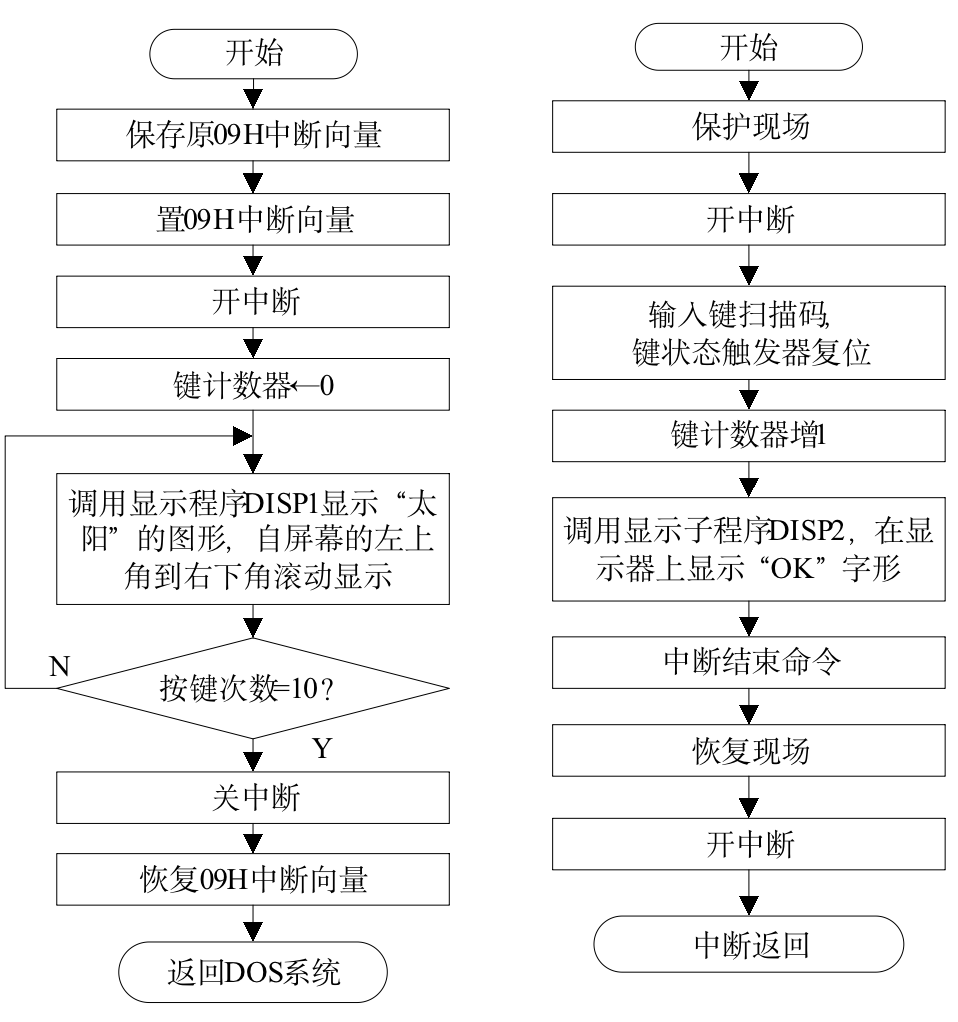
\includegraphics[width=0.7\textwidth]{fig/process.png}
    \caption{任务流程图}
    \label{fig:process}
\end{figure}

在主程序中应先读取并保存中断类型号t的原中断向量,然后再设置新的中断向量,即将中断服务程序\texttt{KEYINTS}入口地址的偏移量和段基址存入以\texttt{09H}$\times$4为起始地址的四个单元内.

在键盘中断程序\texttt{KEYINTS}中,保护现场、开中断之后,就通过8255A的PA口(PA口地址为60H)读取键盘扫描码,接着从\texttt{8255A PB}口 (\texttt{PB}口地址为\texttt{61H})的\texttt{PB7}输出一个正脉冲(即\texttt{PB7}先输出高电平,再输出低电平),先输出的高电平信号反相之后控制键盘状态触发器的清零端,使\texttt{IRQ1}清零,撤消中断请求信号.再输出的低电平信号允许位寄存器输出数据,这样就为传递下一个键盘扫描码作好了准备.

\texttt{8255A PB}口的\texttt{PB7}输出正脉冲来发键盘状态复位命令的具体指令如下:
\begin{lstlisting}[language={[x86masm]Assembler},title=code]
    IN    AL,61H    ;输入PB口的当前值
    OR    AL,80H     ;PB7置1
    OUT   61H,AL
    AND   AL,7FH    ;PB7清零
    OUT   61H,AL
\end{lstlisting}

在键盘中断程序结束前,应发出“中断结束”(\texttt{EOI})命令(控制字为\texttt{20H}),给\texttt{8259A}的操作命令字\texttt{OCW1}(端口地址为\texttt{20H}).具体指令如下:
\begin{lstlisting}[language={[x86masm]Assembler},title=code]
    MOV   AL,20H
    OUT   20H,AL
\end{lstlisting}

然后,实现中断返回.

另外,当键按下时,送向主机的扫描码是键编号,而键释放时,扫描码为键编号加\texttt{80H}(即第7位置1).例如,按下和释放“\texttt{A}”键将向主机发送两个扫描码: \texttt{1EH}和\texttt{9EH}.

以下是主程序中显示“太阳”图形的子程序\texttt{DISP1},仅供参考.
\begin{lstlisting}[language={[x86masm]Assembler},title=code]
    DISP1  PROC  FAR
    PUSH  AX
    PUSH  BX
    PUSH  CX
    PUSH  DX
    MOV   AH,15      ; 读当前显示状态
    INT   10H
    MOV   AH,0       ; 设置显示方式 
    INT   10H
    MOV   DX,0       ; 行号为0,列号为0
    REPT:    
    MOV   AH,2       ; 设置光标位置
    INT   10H
    MOV   AL,0FH     ; 0FH--太阳图形的ASCII码
    MOV   CX,1       ; 显示字符个数
    MOV   AH,10      ; 写字符
    INT   10H
    CALL  DELAY
    SUB   AL,AL      
    MOV   AH,10       ; 清除原图形
    INT   10H
    INC   DH           ; 行号+1
    ADD  DL,2         ; 列号+2
    CMP  DH,25        ; 是否到25行?
    JB   REPT
    POP   DX
    POP   CX
    POP   BX
    POP   AX
    RET
    DISPl  ENDP
\end{lstlisting}

以下是中断服务程序中显示\texttt{OK!}字符子程序\texttt{DISP2},仅供参考.
\begin{lstlisting}[language={[x86masm]Assembler},title=code]
    DISP2  PROC  FAR
    PUSH   CX
    PUSH   BX
    PUSH   AX
    MOV    CX, 3
    NEXTC:LODSB                     ; 字符串"OK!"在数据段中定义,AL←[SI]  
    MOV    AH,0EH            ; 写字符,并移动光标
    MOV    BX,01
    INT    10H
    CALL   DELAY
    LOOP   NEXTC  
    POP    AX
    POP    BX
    POP    CX
    RET
    DISP2  ENDP
\end{lstlisting}

以下是延时1秒子程序:
\begin{lstlisting}[language={[x86masm]Assembler},title=code]
    DELAY PROC   
    PUSH   CX
    PUSH   DX
    MOV    DX,20
    DL500: 
    MOV    CX,2801
    DL10ms:
    LOOP DL10ms
    DEC     DX
    JNZ     DL500 
    POP     DX
    POP     CX
    RET
    DELAY  ENDP
\end{lstlisting}

\section{预备知识}
\begin{note}{\texttt{INT 10H}的\texttt{13H}功能}{}
    \texttt{BH}=页码

    \texttt{BL}=属性(若\texttt{AL}=\texttt{00H}或\texttt{01H})

    \texttt{CX}=显示字符串长度

    (\texttt{DH}、\texttt{DL})=坐标(行、列)

    \texttt{ES:BP}=显示字符串的地址 AL=显示输出方式

    0: 字符串中只含显示字符,其显示属性在BL中.显示后,光标位置不变

    1: 字符串中只含显示字符,其显示属性在BL中.显示后,光标位置改变

    2: 字符串中含显示字符和显示属性.显示后,光标位置不变

    3: 字符串中含显示字符和显示属性.显示后,光标位置改变
\end{note}
\section{实验代码}
% \begin{figure}[htbp]
%     \centering
%     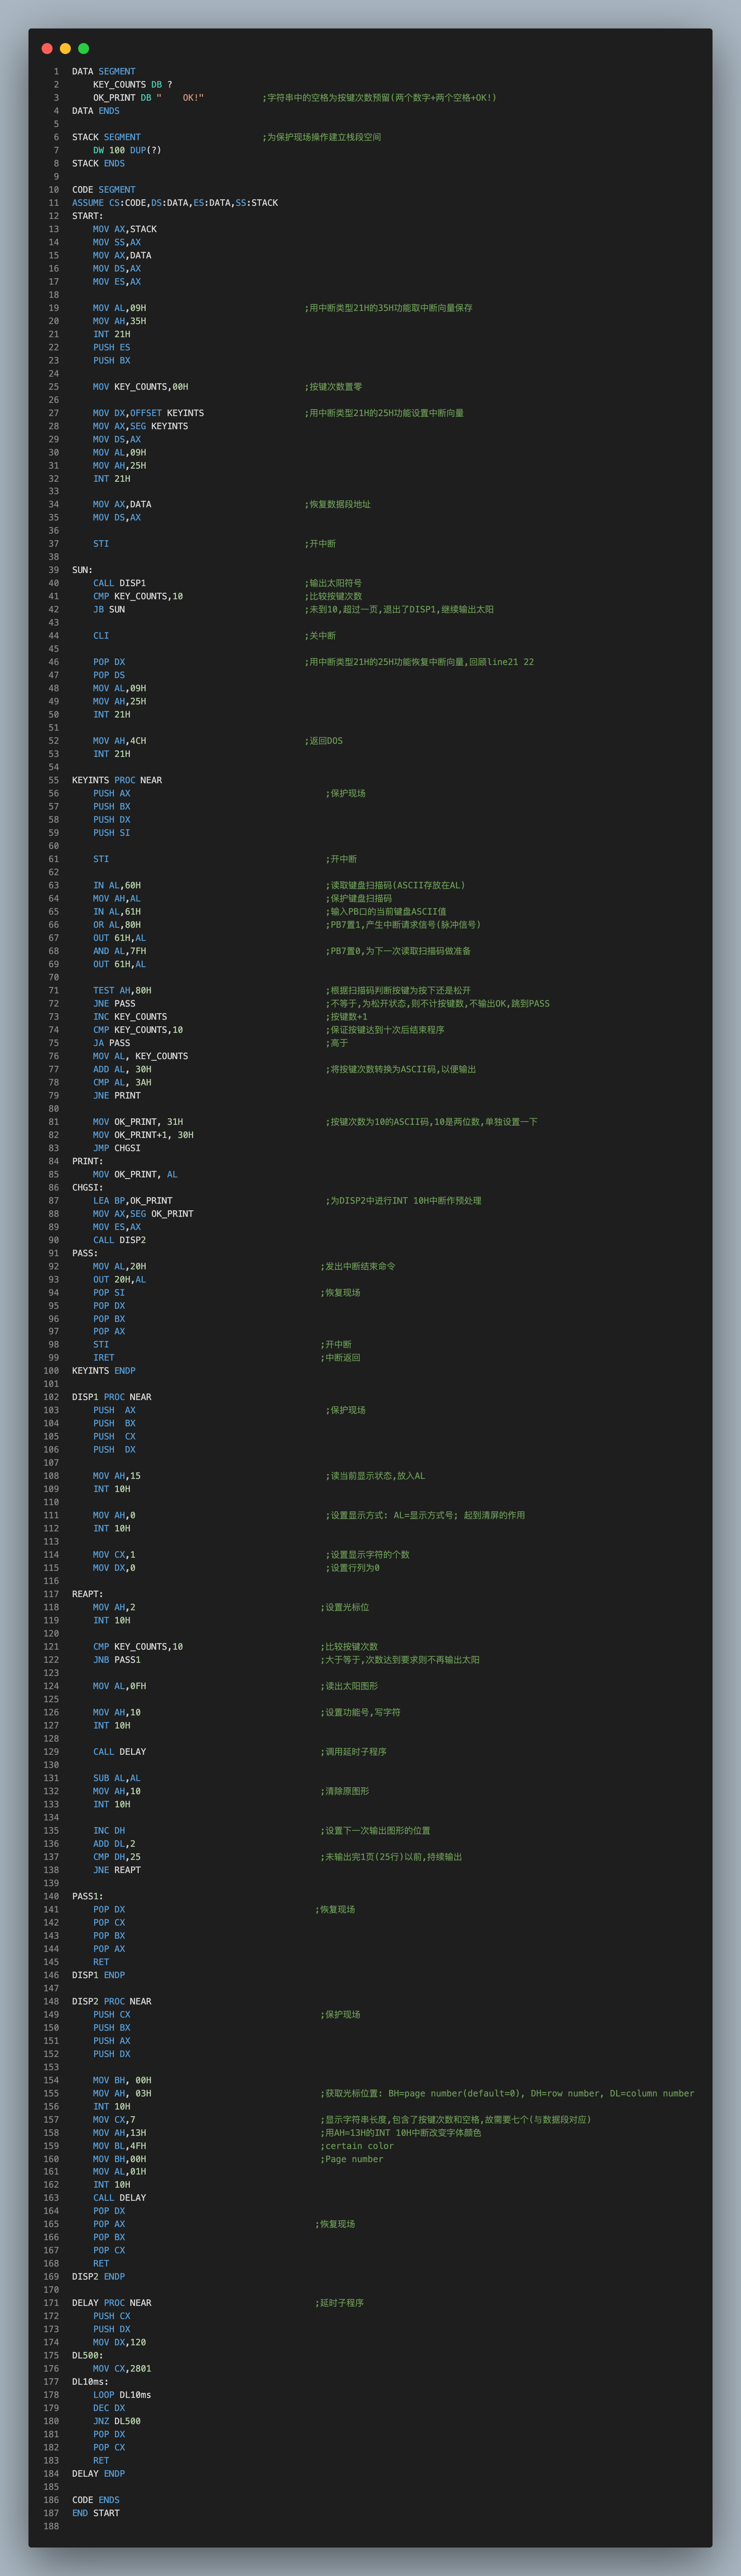
\includegraphics[width=0.7\textwidth]{fig/code.png}
%     \caption{}
%     \label{fig:}
% \end{figure}
\begin{lstlisting}[language={[x86masm]Assembler},title=code]
    DATA SEGMENT
    KEY_COUNTS DB ?
    OK_PRINT DB "    OK!"           ;字符串中的空格为按键次数预留(两个数字+两个空格+OK!)
    DATA ENDS

    STACK SEGMENT                       ;为保护现场操作建立栈段空间
        DW 100 DUP(?)
    STACK ENDS

    CODE SEGMENT
    ASSUME CS:CODE,DS:DATA,ES:DATA,SS:STACK
    START:
        MOV AX,STACK
        MOV SS,AX
        MOV AX,DATA
        MOV DS,AX

        MOV AL,09H                              ;用中断类型21H的35H功能取中断向量保存
        MOV AH,35H
        INT 21H
        PUSH ES
        PUSH BX

        MOV KEY_COUNTS,00H                      ;按键次数置零

        MOV DX,OFFSET KEYINTS                   ;用中断类型21H的25H功能设置中断向量
        MOV AX,SEG KEYINTS
        MOV DS,AX
        MOV AL,09H
        MOV AH,25H
        INT 21H

        MOV AX,DATA                             ;恢复数据段地址
        MOV DS,AX

        STI                                     ;开中断

    SUN:
        CALL DISP1                              ;输出太阳符号
        CMP KEY_COUNTS,10                       ;比较按键次数
        JB SUN                                  ;未到10,超过一页,退出了DISP1,继续输出太阳

        CLI                                     ;关中断

        POP DX                                  ;用中断类型21H的25H功能恢复中断向量,回顾line21 22
        POP DS
        MOV AL,09H
        MOV AH,25H
        INT 21H                            

        MOV AH,4CH                              ;返回DOS
        INT 21H

    KEYINTS PROC NEAR
        PUSH AX                                     ;保护现场
        PUSH BX
        PUSH DX
        PUSH SI

        STI                                         ;开中断

        IN AL,60H                                   ;读取键盘扫描码(ASCII存放在AL)
        MOV AH,AL                                   ;保护键盘扫描码               
        IN AL,61H                                   ;输入PB口的当前键盘ASCII值
        OR AL,80H                                   ;PB7置1,产生中断请求信号(脉冲信号)
        OUT 61H,AL
        AND AL,7FH                                  ;PB7置0,为下一次读取扫描码做准备
        OUT 61H,AL

        TEST AH,80H                                 ;根据扫描码判断按键为按下还是松开
        JNE PASS                                    ;不等于,为松开状态,则不计按键数,不输出OK,跳到PASS
        INC KEY_COUNTS                              ;按键数+1
        CMP KEY_COUNTS,10                           ;保证按键达到十次后结束程序
        JA PASS                                     ;高于
        MOV AL, KEY_COUNTS
        ADD AL, 30H                                 ;将按键次数转换为ASCII码,以便输出
        CMP AL, 3AH
        JNE PRINT

        MOV OK_PRINT, 31H                           ;按键次数为10的ASCII码,10是两位数,单独设置一下
        MOV OK_PRINT+1, 30H
        JMP CHGSI
    PRINT:  
        MOV OK_PRINT, AL
    CHGSI:  
        LEA BP,OK_PRINT                             ;为DISP2中进行INT 10H中断作预处理
        MOV AX,SEG OK_PRINT                        
        MOV ES,AX
        CALL DISP2
    PASS:
        MOV AL,20H                                 ;发出中断结束命令
        OUT 20H,AL
        POP SI                                     ;恢复现场
        POP DX
        POP BX
        POP AX
        IRET                                       ;中断返回
    KEYINTS ENDP

    DISP1 PROC NEAR
        PUSH  AX                                    ;保护现场
        PUSH  BX
        PUSH  CX
        PUSH  DX

        MOV AH,15                                   ;读当前显示状态,放入AL
        INT 10H

        MOV AH,0                                    ;设置显示方式: AL=显示方式号; 起到清屏的作用
        INT 10H

        MOV CX,1                                    ;设置显示字符的个数
        MOV DX,0                                    ;设置行列为0

    REAPT:
        MOV AH,2                                   ;设置光标位
        INT 10H

        CMP KEY_COUNTS,10                          ;比较按键次数
        JNB PASS1                                  ;大于等于,次数达到要求则不再输出太阳

        MOV AL,0FH                                 ;读出太阳图形

        MOV AH,10                                  ;设置功能号,写字符
        INT 10H

        CALL DELAY                                 ;调用延时子程序

        SUB AL,AL
        MOV AH,10                                  ;清除原图形
        INT 10H

        INC DH                                     ;设置下一次输出图形的位置
        ADD DL,2                                    
        CMP DH,25                                  ;未输出完1页(25行)以前,持续输出
        JNE REAPT

    PASS1:
        POP DX                                    ;恢复现场
        POP CX
        POP BX
        POP AX
        RET
    DISP1 ENDP

    DISP2 PROC NEAR
        PUSH CX                                    ;保护现场
        PUSH BX
        PUSH AX
        PUSH DX

        MOV BH, 00H                                
        MOV AH, 03H                                ;获取光标位置: BH=page number(default=0), DH=row number, DL=column number
        INT 10H
        MOV CX,7                                   ;显示字符串长度,包含了按键次数和空格,故需要七个(与数据段对应)
        MOV AH,13H                                 ;用AH=13H的INT 10H中断改变字体颜色
        MOV BL,4FH                                 ;certain color
        MOV BH,00H                                 ;Page number
        MOV AL,01H
        INT 10H                                   
        CALL DELAY
        POP DX
        POP AX                                    ;恢复现场
        POP BX
        POP CX
        RET
    DISP2 ENDP

    DELAY PROC NEAR		                          ;延时子程序
        PUSH CX
        PUSH DX
        MOV DX,120
    DL500:
        MOV CX,2801
    DL10ms:
        LOOP DL10ms
        DEC DX
        JNZ DL500
        POP DX
        POP CX
        RET
    DELAY ENDP

    CODE ENDS
    END START

\end{lstlisting}

\section{附加任务阐述}
\subsection{附加任务1}
任务代码如图\ref{fig:task1}.
\begin{figure}[htbp]
    \centering
    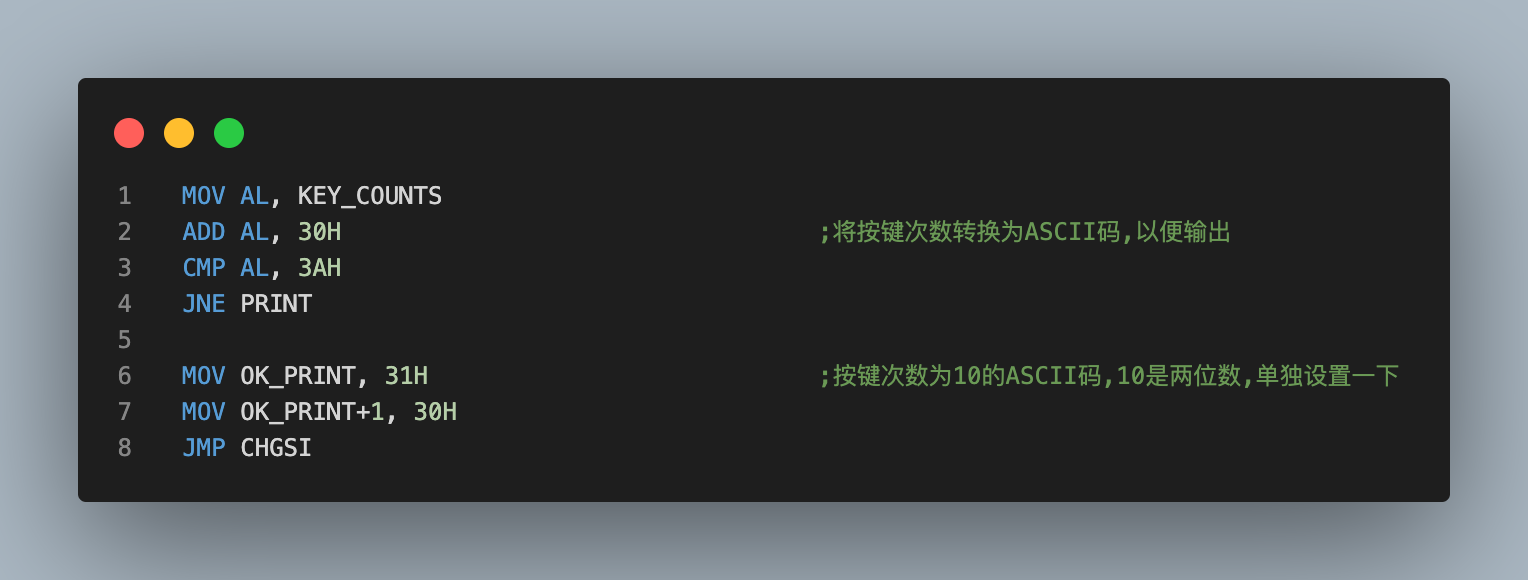
\includegraphics[width=0.7\textwidth]{fig/task1.png}
    \caption{附加任务1}
    \label{fig:task1}
\end{figure}

\subsection{附加任务2}
任务代码如图\ref{fig:task2}.
\begin{figure}[htbp]
    \centering
    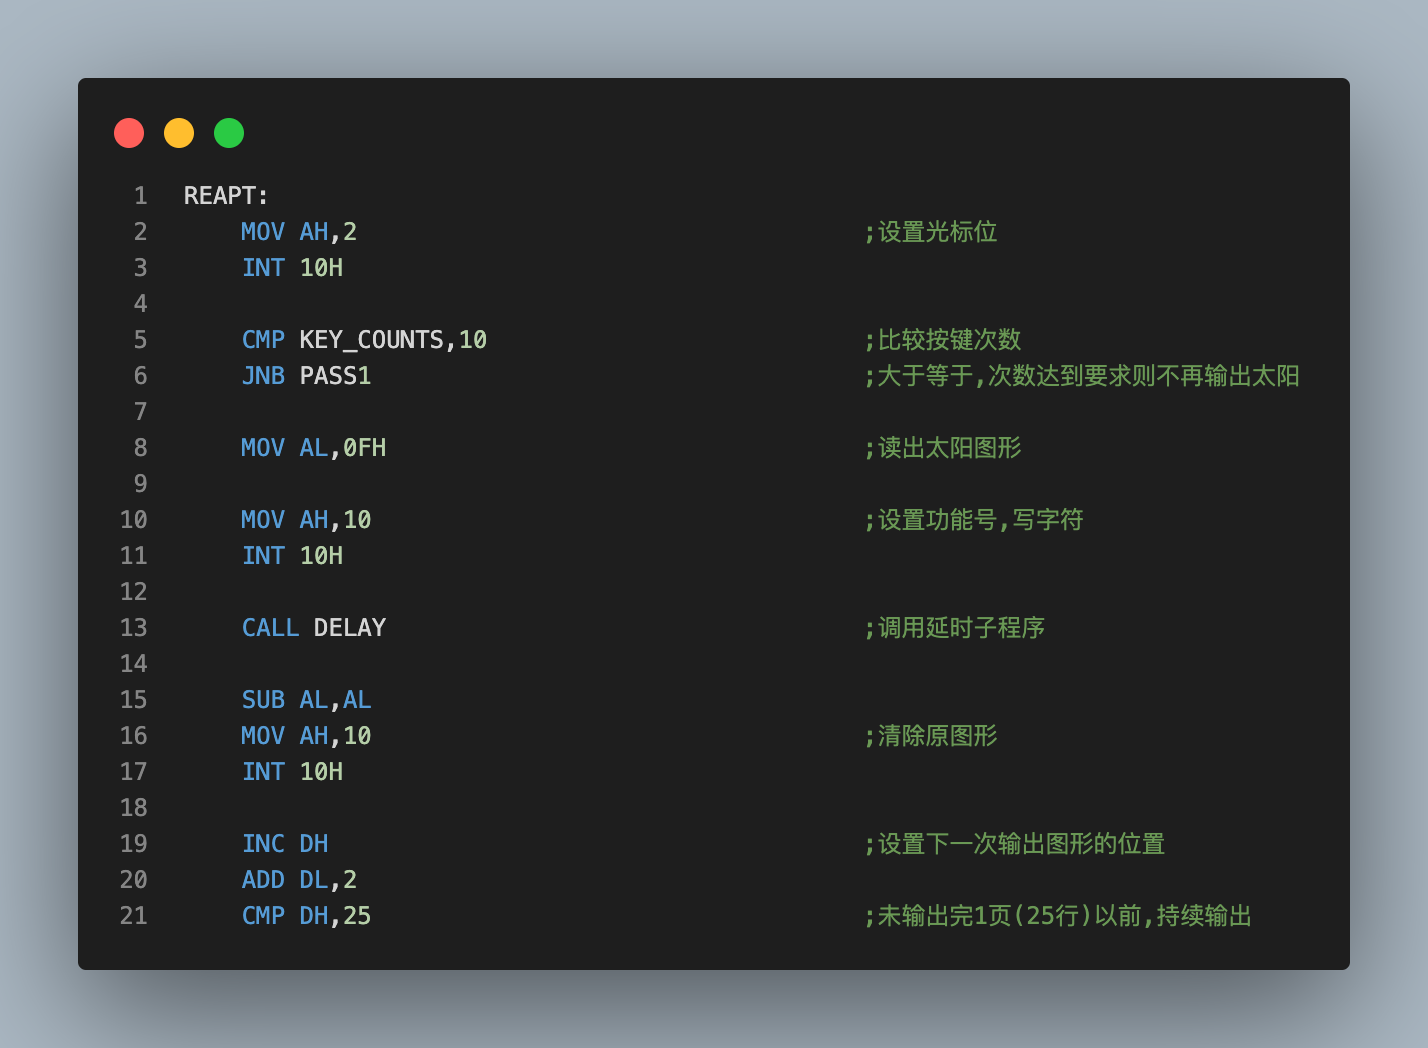
\includegraphics[width=0.7\textwidth]{fig/task2.png}
    \caption{附加任务2}
    \label{fig:task2}
\end{figure}

\subsection{附加任务3}
任务代码如图\ref{fig:task3}.
\begin{figure}[htbp]
    \centering
    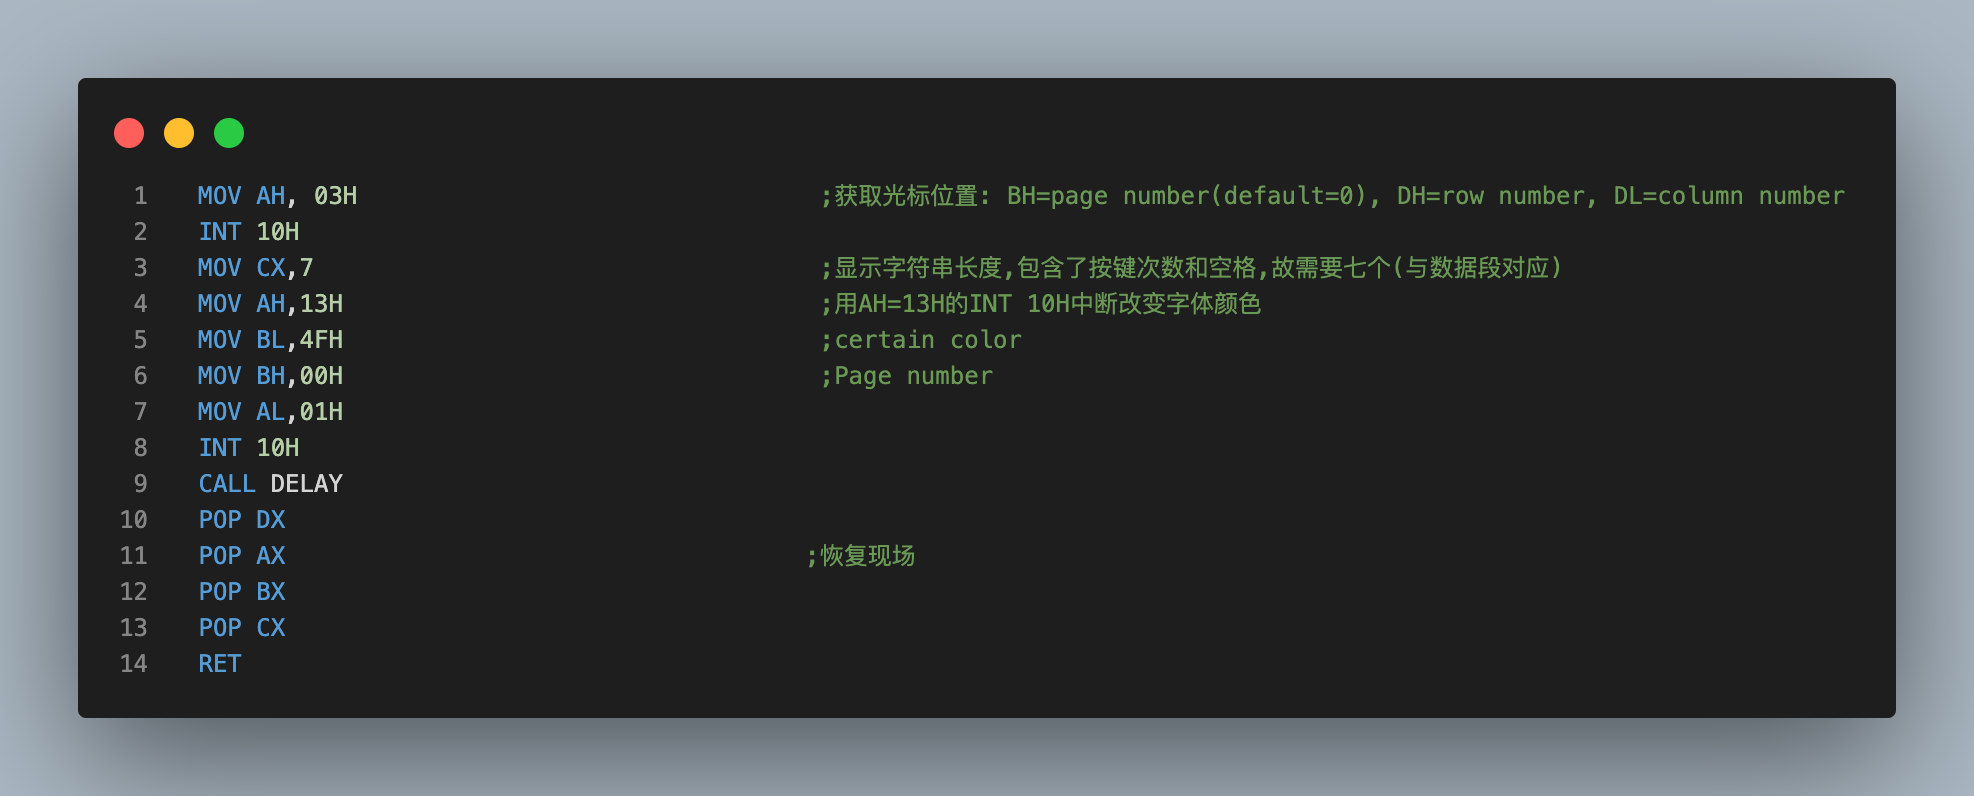
\includegraphics[width=0.7\textwidth]{fig/task3.png}
    \caption{附加任务3}
    \label{fig:task3}
\end{figure}

\section{结果验证}
运行程序,按键10次后效果图如图 \ref{fig:rlt}
\begin{figure}[htbp]
    \centering
    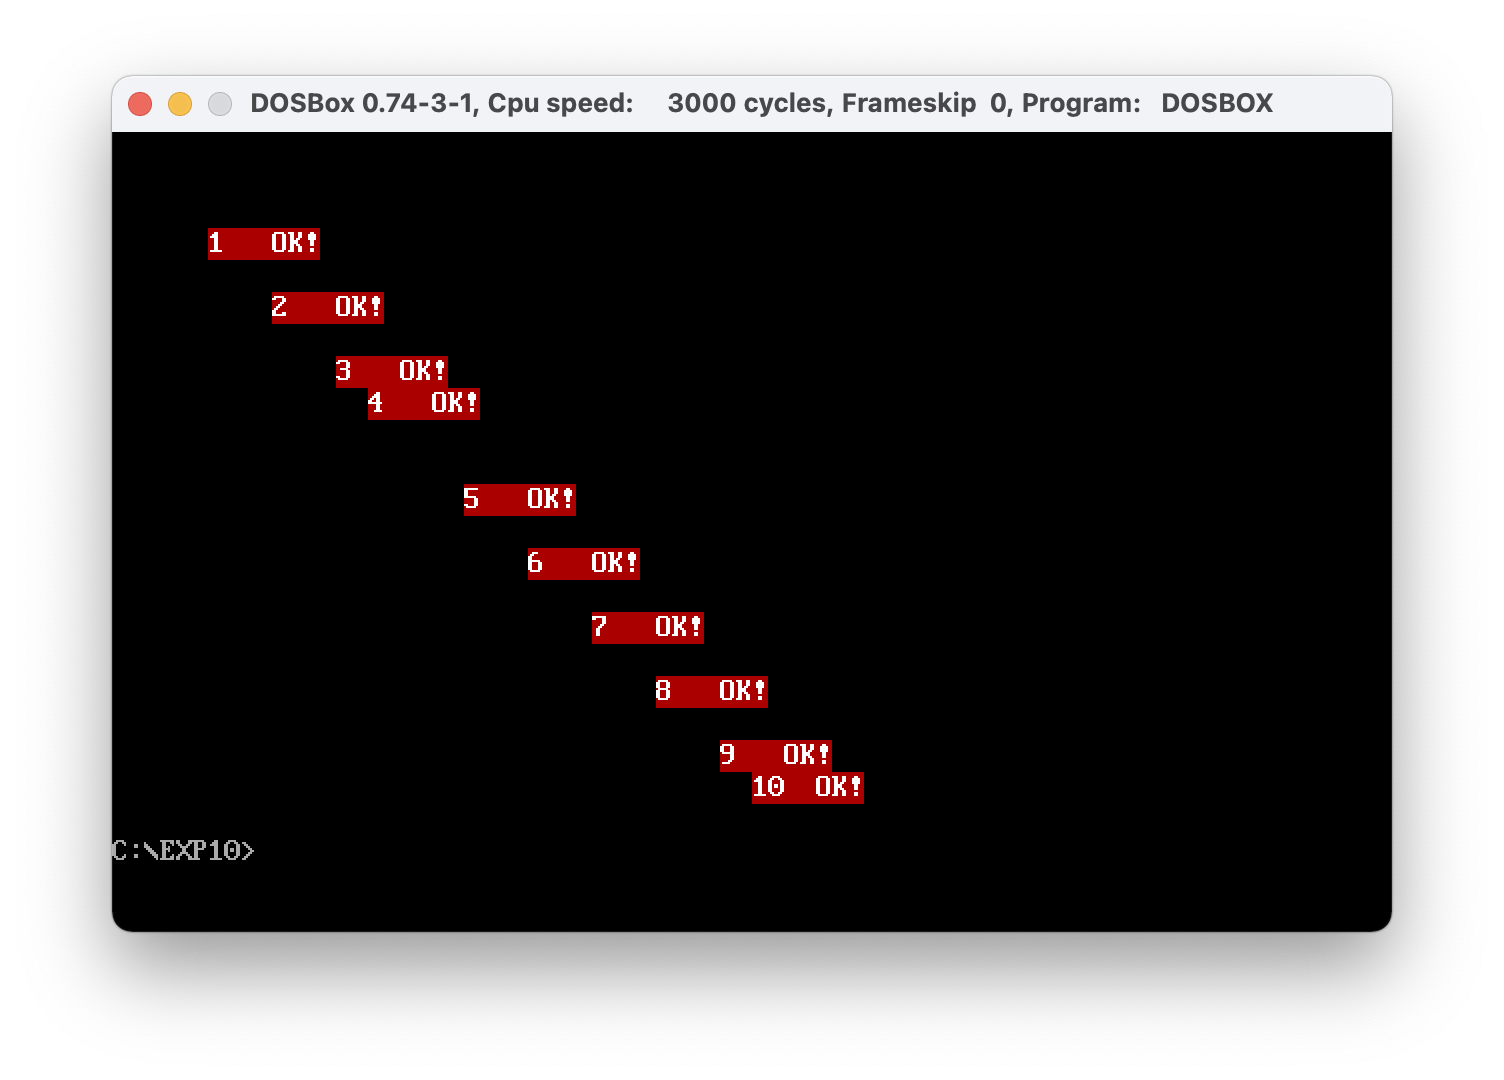
\includegraphics[width=0.7\textwidth]{fig/rlt.png}
    \caption{}
    \label{fig:rlt}
\end{figure}

\section{思考题}
\textcolor{red}{键盘上某个键按下和释放时都会向\texttt{8259}发出中断请求,要求只在键按下时显示\texttt{OK!},键释放时不显示,则中断服务程序\texttt{KEYINTS}应如何修改?}

可以根据键盘上按键按下和释放时的键盘扫描码第七位不同,进而判断按键的状态,具体操作如下: 读取键盘扫描码\texttt{IN AL,60H}后保留\texttt{MOV AH,AL},之后根据扫描码的第七位\texttt{TEST AH,80H}: 是0则为按下状态,计数加1并输出\texttt{OK!};是1则为松开,不再计数及输出\texttt{OK!}(\texttt{JNZ PASS})。这样即可实现要求功能.

\section{实验总结}
\begin{enumerate}
    \item 在实现附加功能四,即修改字符的属性时,起初想要利用功能号为\texttt{09H}的\texttt{INT 10H}中断,但是按照\texttt{INT 10H}中断操作设置不同颜色后,输出的字符始终是黑白色。经过不断的调研,发现功能号为\texttt{09H}的\texttt{INT 10H}中断中,若要设置字符颜色和背景颜色,需要在图形模式下进行,但是本实验其他功能的实现需要在文本模式下实现,于是无法使用功能号为\texttt{09H}的\texttt{INT 10H}中断。调研后发现可以用功能号为\texttt{13H}的\texttt{INT 10H}中断(输出字符串)代替功能号为\texttt{09H}的\texttt{INT 10H}中断,且该中断设置颜色时没有工作模式限制,于是,使用功能号为\texttt{13H}的\texttt{INT 10H}中断终于实现了设置字符颜色和背景颜色的功能.
    \item 在实现附加功能二的过程中,起初观察到输出的\texttt{OK!}字符不全,发现原因是字符串长度改变,但进行\texttt{INT 10H}中断时未调整\texttt{CH}。调整后解决了问题.
    \item 实验任务流程图中右图倒数第二行所给的最后一个开中断没有用,应去除.
    \item 其他实验总结已随文附在“注意”、“思考、“分析”中。
\end{enumerate}



% 打印参考文献
\addcontentsline{toc}{section}{参考文献}
\printbibliography

\end{document}
